\documentclass[10pt,aspectratio=169,handout]{beamer}

\usepackage[utf8]{inputenc}
\usepackage[ngerman]{babel}
\usepackage{utopia}
\usetheme{Darmstadt}
\usecolortheme{default}
\usepackage{xcolor}
\usepackage{graphicx}
\usepackage{amsmath}
\usepackage{amsthm}
\usepackage{amssymb}
\usepackage{amsfonts}
\usepackage{mathtools}
\usepackage{dsfont}
\usepackage{hyperref}
\usepackage[most]{tcolorbox}
\usepackage{tikz}
\usepackage{adjustbox}
\usepackage{mathrsfs}
\usepackage{minted}
\usetikzlibrary{cd}
\usetikzlibrary{positioning}
\usetikzlibrary{calc}
\usetikzlibrary{arrows.meta}
\setbeamertemplate{theorems}[numbered]
\setbeamertemplate{navigation symbols}{}
\newtranslation[to=ngerman]{Theorem}{Satz}
\def\C{\mathbb{C}}
\def\R{\mathbb{R}}
\def\Q{\mathbb{Q}}
\def\N{\mathbb{N}}
\def\Z{\mathbb{Z}}
\def\cA{\mathcal{A}}
\definecolor{LightGray}{gray}{0.9}


\begin{document}

\title{Principles of Machine Learning: Exercise 4}
\date{18.12.2023}
\author{Alina Pollehn (3197257), Julian Litz (3362592), Manuel Hinz (3334548)\\
    Felix Göhde (3336445), Felix Lehmann (3177181), Caspar Wiswesser (3221493)\\
    Adrian Köring (3347785), Greta Günther (3326765), Linus Mallwitz (3327653)\\
    Niklas Mueller-Goldingen (3363219), Jennifer Kroppen (2783393)}

\begin{frame}
    \maketitle
\end{frame}

\section{Exercise 4.1}

\begin{frame}

    \frametitle{Exercise 4.1: Overview}

    \begin{enumerate}
        \item Goal: Minimize $f(\mu)\coloneqq \frac{1}{n}\sum_{j=1}^{n} \Vert x_j-\mu\Vert$
        \item Alternative formulation: Find $w\geq 0$ s.t. $1^\intercal w=1$ and \[w=\argmin_w\underbrace{\frac{1}{n}\sum_{j=1}^n \Vert x_j - Xw \Vert^2}_{\eqqcolon g(w)}\]
        \item We want to use the Frank-Wolfe algorithm to solve our optimization problem, therefore we also need the gradient: \[\nabla g = 2 X^\intercal X [w-\frac{1}{n}1]\]
    \end{enumerate}

\end{frame}

\begin{frame}
    \frametitle{Exercise 4.1: Implementation}

    \inputminted[bgcolor=LightGray,fontsize=\small]{python}{code/ex4-1.py}

\end{frame}

\begin{frame}
    \frametitle{Exercise 4.1: Error analysis}

    Because we know the minimizer (which is just the mean of our vectors), we can calculate our error $\epsilon \coloneqq \Vert \hat{\mu}-\mu\Vert$
    as a function of the number of iterations. We also know that the error should be in $O(\frac{1}{T})$.

    \begin{minipage}{0.49\textwidth}
        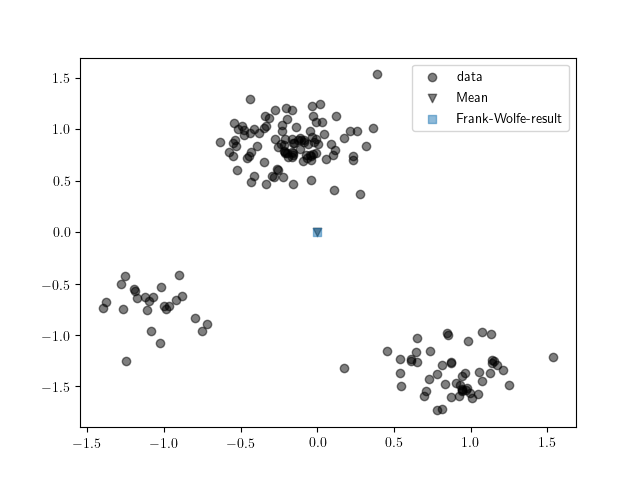
\includegraphics[width=\textwidth]{images/10000.png}
    \end{minipage}
    \begin{minipage}{0.49\textwidth}
        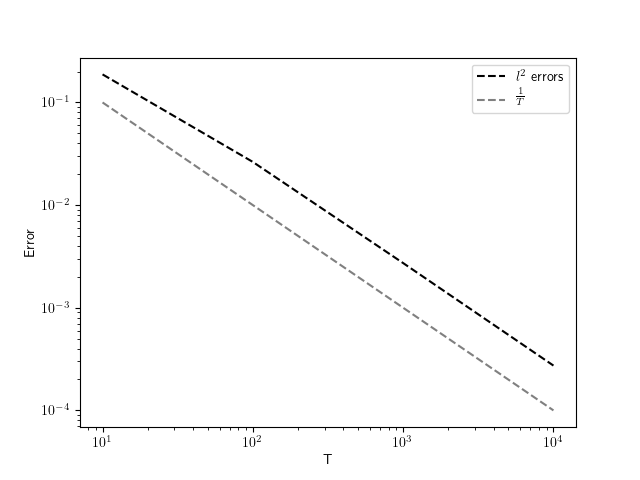
\includegraphics[width=\textwidth]{images/errors.png}
    \end{minipage}

    We also ran least squares to estimate the exponent similarly to Task 1-3. This yields $-1.05 \approx -1$, which also 
    consistent with our theoretical error bound.

\end{frame}

\section{Exercise 4.2}

\begin{frame}
    \frametitle{Exercise 4.2: Proving two identities}

    Let $X$ be our data matrix and $w=\frac{1}{n}1_n$ and $z\in \R^n$. 

    Then the following identities hold:

    \begin{equation*}
        \tr[\overbrace{X^\intercal X}^{A_1} w z^\intercal] = z^\intercal X^\intercal X w
    \end{equation*}
    \begin{equation*}
        \tr[\underbrace{zw^\intercal X^\intercal X}_{A_2} w z^\intercal] = z^\intercal z \cdot w^\intercal X^\intercal X w=z^\intercal (zw^\intercal X^\intercal X) w
    \end{equation*}  

    It suffices to show the following lemma (using either $A=A_1$ or $A=A_2$):

    \begin{lemma}
        For a matrix $A\in \R^{n\times n},w=\frac{1}{n}1_n\in \R^n$ and $z\in R^n$ the following equality holds:
        \[\tr(Awz^\intercal)=z^\intercal A w\]
    \end{lemma}

\end{frame}

\begin{frame}
    \frametitle{Proof of Lemma 1}

    \begin{proof}
        \begin{enumerate}
            \item First we use $\tr(A \overbrace{wz^\intercal}^{\in \R^{n\times n}})=\tr(wz^\intercal A)$ (because we apply a cyclic permutation)
            \item Now $a\coloneqq z^\intercal A$ is just a row vector, therefore 
            \begin{align*}
                w a &= \begin{pmatrix}
                    \frac{a_1}{n} & \dots & \frac{a_n}{n}\\
                    \vdots &\vdots&\vdots\\
                    \frac{a_1}{n} & \dots & \frac{a_n}{n}
                \end{pmatrix}\in\R^{n\times n}\\
                \implies \tr(wa)&=\sum_{i=1}^n \frac{a_i}{n} = \sum_{i=1}^n \frac{a_i}{n} \cdot 1 = \sum_{i=1}^{n}a_i \frac{(1_n)_i}{n}\\
                & = (z^T A)w
            \end{align*}
        \end{enumerate}
        
    \end{proof}

\end{frame}


\section{Exercise 4.3}

\begin{frame}
    \frametitle{Exercise 4.3: Creative Farthest Points}

    Select $\mathcal{X} = \{x_1, x_2, \dots, x_n \}$ maximizing $\hat{S} = \underset{S \subset \mathcal{X}}{\mathrm{argmax}}  \underset{x_i \in S}\sum \underset{x_j \in S}\sum || x_i - x_j||^2$ s.t. $|S| = k$

    Problem
    \begin{itemize}
        \item NP-hard problem with the number of possible solutions in ${N\choose k}$
        \item e.g. for the largest choice of $k=100$ with the face dataset: ${2429\choose 100} = 4.73 \cdot 10^{179}$ 
    \end{itemize}
\end{frame}

\begin{frame}
    \frametitle{Farthest-First Traversal}
    Heuristical-approach to an approximate solution
    \begin{enumerate}
        \item Sample seed point randomly $\hat{S} = \{ x_0 \}$
        \item Iteratively add the point that is furthest from all points in $\hat{S}$

        More specifically: 
        \begin{enumerate}
            \item Determine distance $x_j$ to all points in $\hat{S}$ $\rightarrow$ remember smallest $d(x_j, \hat{S})$ over subset
            \item Add $x_j$ with largest distance $d(x_j, \hat{S})$ over $x_j  \in \mathcal{X}$
            \item Repeat until $|\hat{S}| = k$
        \end{enumerate}
    \end{enumerate}
\end{frame}

\begin{frame}
    \inputminted[bgcolor=LightGray,fontsize=\small]{python}{code/farthest-first.py}
\end{frame}


\section{Exercise 4.4}

\begin{frame}
    \frametitle{$k$-means clustering: Two perspectives}

    \begin{enumerate}
        \item well known formulation: Minimize:\[\mu_1,\dots,\mu_k=\argmin_{\mu_1,\dots,\mu_k} \sum_{i=1}^k\sum_{x_j\in C_i} \Vert x_j-\mu_i\Vert^2\]
        where $(C_i)_i$ are the clusters and $\mu_i$ are the centroids of each cluster.
        \item Alternative formulation: \[\mu_1,\dots,\mu_k=\argmin_{\mu_1,\dots,\mu_k} \sum_{i=1}^k\sum_{x_j\in C_i} z_{ij}\Vert x_j-\mu_i\Vert^2\]
        where $z_{ij}\in\{0,1\}$ and $\sum_{i=1}^{k}z_{ij}=1$
        \item  The second formulation can be solved by a Frank-Wolfe-procedure:
    \end{enumerate}

\end{frame}

\begin{frame}

    \inputminted[bgcolor=LightGray,fontsize=\small]{python}{code/fw_kmeans_v1.py}
    \vspace{-5mm}
    \inputminted[bgcolor=LightGray,fontsize=\small]{python}{code/fw_update_z.py}

\end{frame}

\begin{frame}
    \frametitle{Exercise 4.4.1: Results}
    \begin{minipage}{0.49\textwidth}
        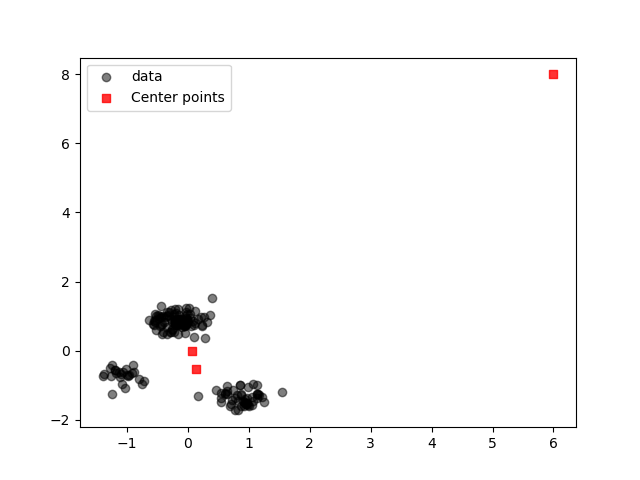
\includegraphics[width=\textwidth]{images/kmeans-n.png}+
        \captionof{figure}{Result of the naive algorithm}
    \end{minipage}
    \begin{minipage}{0.49\textwidth}
        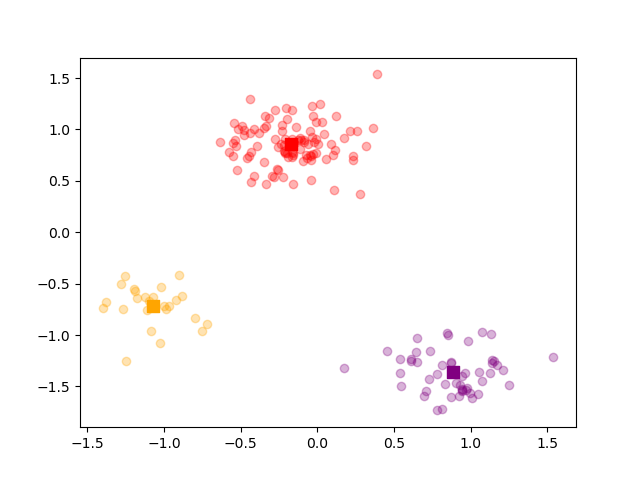
\includegraphics[width=\textwidth]{images/blob_mean4.4.png}
        \captionof{figure}{Result of FW-$k$-means Version 1}
    \end{minipage}

    Clearly the results of the naive algorithm are worthless, while also crashing considerably more!
\end{frame}

\begin{frame}
    \frametitle{Exercise 4.4.2: Results}
    \begin{minipage}{0.49\textwidth}
        \begin{enumerate}
            \item While using random data points to construct $M$ causes stability issues,because of two matrix inversions, these were manageable
            \item Given that our solution for Exercise 4.3 is still rather slow for large $k$, it was still faster 
            to use random, rather than maximally different, data points.
        \end{enumerate}
    \end{minipage}    
    \begin{minipage}{0.49\textwidth}
        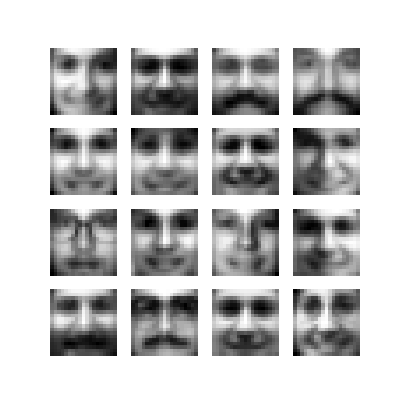
\includegraphics[width=0.85\textwidth]{images/faces_mean4_4.png}
        \captionof{figure}{Result of FW-$k$-means Version 1}
    \end{minipage}

\end{frame}

\section{Exercise 4.5}

\begin{frame}
    \frametitle{Exercise 4.5: }

    \begin{enumerate}
        \item Code is very similar to exercise 4.4:
        \begin{itemize}
            \item uses the same vectorization to get rid of the for-loop
            \item uses random data points to generate $M$ before the first iteration 
        \end{itemize}
        \item Main difference: no matrix inversion $\implies$ more robust
        \item Similar results: comparable difference when comparing both, or two results of the same version 
    \end{enumerate}
    

\end{frame}

\begin{frame}
    \frametitle{Exercise 4.5: Results}

    \begin{minipage}{0.49\textwidth}
        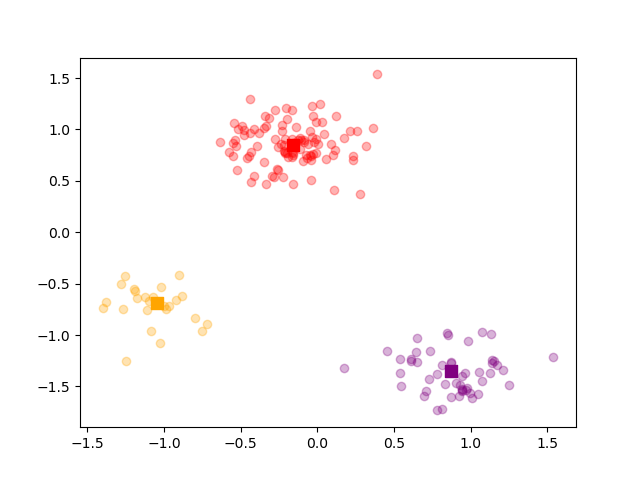
\includegraphics[width=\textwidth]{images/blob_4_5.png}
        \captionof{figure}{Result of FW-$k$-means Version 2 for threeBlobs.csv}
    \end{minipage}
    \begin{minipage}{0.49\textwidth}
        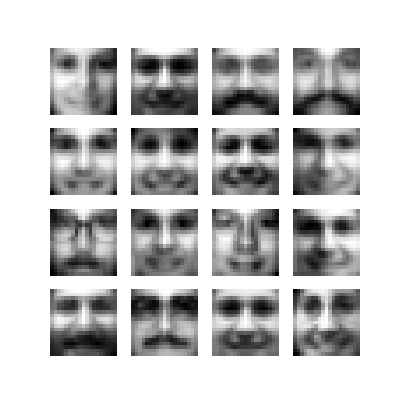
\includegraphics[width=0.85\textwidth]{images/faces_4_5.png}
        \captionof{figure}{Result of FW-$k$-means Version 2 for faceMatrix.npy}
    \end{minipage}
   

\end{frame}

\section{Exercise 4.6}

\begin{frame}
    \frametitle{Exercise 4.6: Comparisson}

    \begin{minipage}{0.34\textwidth}
        \begin{enumerate}
            \item Similar optimization problem compared to exercise 4.5: We only drop the constraint \[Z\in \{0,1\}^{k\times n}\]
            \item Similar code to exercise 4.5
            \item Result: We get a set of "exaggerated" representations for each cluster, rather than the mean of each cluster
        \end{enumerate}
    \end{minipage}    
    \begin{minipage}{0.65\textwidth}
        \inputminted[bgcolor=LightGray,fontsize=\small]{python}{code/fw_archetypal_analysis.py}
    \end{minipage}
\end{frame}

\begin{frame}
    \frametitle{Exercise 4.6: Results}

    \begin{minipage}{0.49\textwidth}
        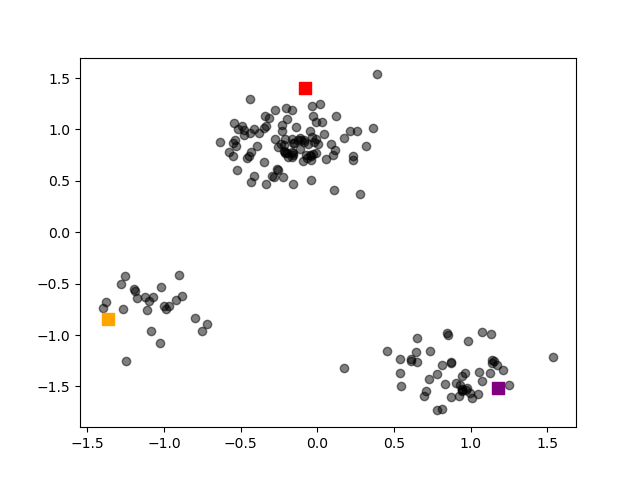
\includegraphics[width=\textwidth]{images/blob_4_6.png}
        \captionof{figure}{Archetypes of threeBlobs.csv}
    \end{minipage}
    \begin{minipage}{0.49\textwidth}
        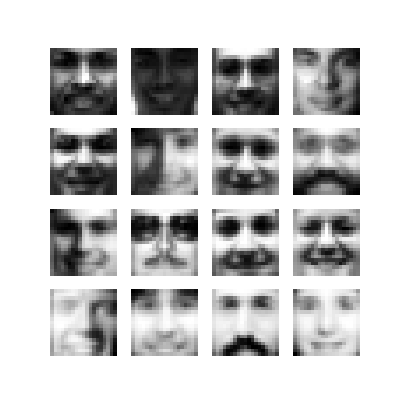
\includegraphics[width=0.85\textwidth]{images/faces_4_6.png}
        \captionof{figure}{Archetypes of faceMatrix.npy}
    \end{minipage}
   

\end{frame}

\end{document}
